%!TEX root = ../../main.tex
\section{Administration Tools}\label{sec:impAdminTools}
% This section describes the administrative functionality. 
% It covers route history, GPS history, bicycle usage history, and an add/remove page.
% It also contains a bicycle GPS tracking, but this has been mentioned in \secref{sec:googlemapsapi}.
In \secref{sec:designAdminTools} a list of questions were made and explained, setting out requirements or guidelines for the features of the administration tools, in that an administrator should be able to answer the questions using these tools. 
In this section we describe how to answer the questions from \secref{sec:designAdminTools} with a visual presentation of the relevant data.

To answer the question about `which routes are used' we implemented a feature to show route history, which can be seen in \secref{sec:routeHistory}.
`Hotspot detection' was not implemented, but GPS history was implemented in \secref{sec:gpsHistory}.
The `traffic of bicycles during some period' can be seen using the chord diagram in \secref{sec:bicycleUsageHistory}
How the `amount of bicycles at a station change over time' can be seen in the `line diagram' from  \secref{sec:bicycleUsageHistory}.

\subsection{Route History}\label{sec:routeHistory}
This part of the administration site handles showing a map of the historical locations of a bicycle.
The administrator provides one or more bicycles, a start, and end date.
Then if there are historical GPS coordinates for the bicycle(s), they will be shown on the map. 

The purpose of the route history page is to give the administrators an idea of which roads the bicycles are traveling a lot on. 
This can then be used as a decision-making tool to decide where to put new stations, in that if the administrator can see that a lot of bicycles are traveling to a specific point it might be a good idea to put a station there.
It could also be used to see if a specific bicycle is being 'misused' in the sense that it would be visible if the bicycle is only being used to travel to one spot and nowhere else.

See \figref{fig:routehistory} for a figure of what the page looks like.

\begin{figure}[H]
	\centering
	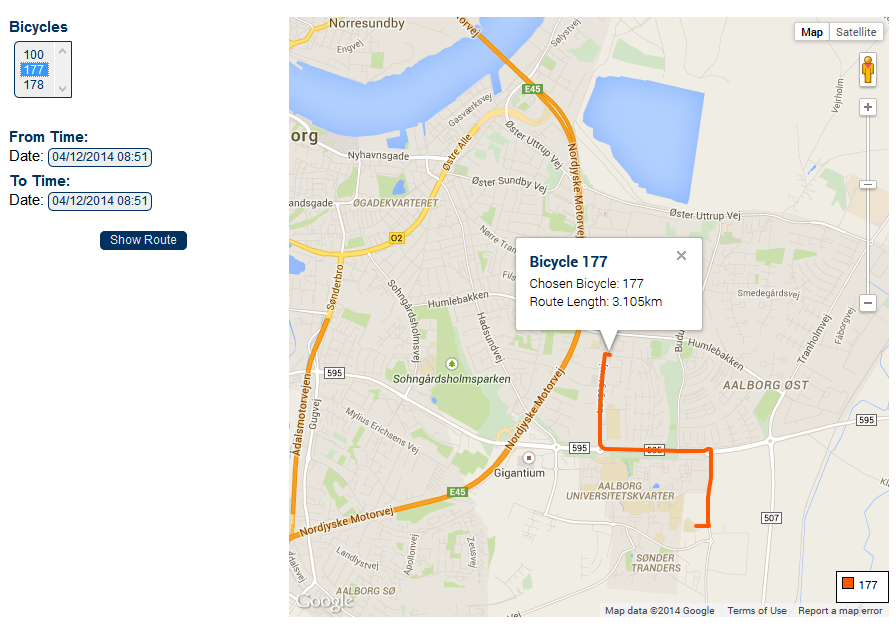
\includegraphics[scale=0.5]{RouteHistory.png}
	\caption{Picture of Route History}
	\label{fig:routehistory}
\end{figure}

From the figure, the presentation of routes are shown for the bicycles with id 36 and 95.

The reason multiple bicycles can be selected is to enable the administrator to compare routes on the same map, this includes the route polyline, chosen bicycle and length,


This feature will make use of the historyusagelocation table designed and implemented, showing the coordinates from the table in a map.
The table is inserted into by the gpsregister interface described in \secref{sec:architecture}.
It is implemented by finding all the bicycles that have associated historical GPS data.
The administrator then chooses which bicycles to map, and these bicycles then have their routes loaded which are then given to Google Maps API to display as a polyline.

\subsection{GPS History}\label{sec:gpsHistory}
From the previous administration feature a historyusagelocation table was implemented to store the positions of a bicycle.
This can also be used to find the last known location of the bicycle. 
This would allow the administrator to determine where missing bicycles are, which in turn would allow for easier recovery of bicycles.

%At the same time when location is recorded from a service, it needs to also record it permanently in the global database.




\subsection{Bicycle Usage History}\label{sec:bicycleUsageHistory}
% Disposition:
% What does it track?
% Which questions can be answered?
% How is it implemented?

Besides recording the exact location of each bicycle with GPS coordinates, the system also records the stations a given bicycle visits.
This information is stored in the historyusagebicycle table implemented from \secref{sec:designAdminTools}.
Information is inserted into this table based on events happening at the stations. 
Every time a bicycle is taken from a dock at a station the stationtodbregister interface is contacted, which takes care of inserting the information about the start station of the trip.
Furthermore every time a bicycle is returned to a station the interface takes care of updating the trip with an end station.
Keeping such information about a bicycle trip can be used to give an overview of the bicycle traffic between stations.

The amount of docked bicycles is tracked for each station, giving an overview of which stations that have high and low activity.
This is implemented through the historyusagestation table described in \secref{sec:designAdminTools}, storing the amount of bicycles at each station.
The insertion is event-based and happens every time a bicycle is either returned to or taken from a station, again through the stationtodbregister interface described in \secref{sec:architecture}.

% line diagram
For illustration the current amount of bicycles at a station and how the amount changes over time, a line diagram is generated showing time on the x-axis and the amount of bicycles on the y-axis, see \figref{fig:linediagram}.
%Insert figure here showing the line diagram.
\begin{figure}[h]
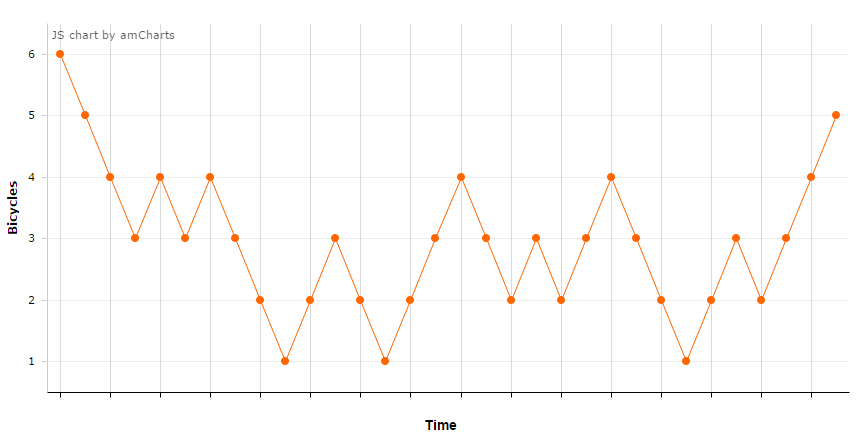
\includegraphics[scale=0.5]{implementation/linediagram}
\caption{Line diagram showing the amount of bicycles.}\label{fig:linediagram}
\end{figure}

% chord diagram
To illustrate the traffic between stations we use a chord diagram. 
An example of this diagram can be seen in \figref{fig:chorddiagram}. 
The input to the diagram is a list of station names and a $n \times n$ matrix where $n$ is the number of stations and where each entry $e_{i,j}$ is a number of bicycles travelling from station $i$ to station $j$. 
Each block at the edge of the diagram represents a station. 
The wider the block, the more bicycles have left that station. 
Each arc of the same colour as the block it is connected to, indicates the number of bicycles leaving the station and the destination of the bicycles. 
The width of the arc at each end shows how many bicycles have travelled in each direction between the two stations. 
For example the red one in the top between the two blue blocks shows that bicycles leaving have travelled to two different destinations. 
As seen from the table on the right, one bicycle went to Karolinelund, and one to Strandvejen. 
Since the arc is narrow at the destination block it means that no bicycle went the other way. 
In some cases the arc destination is somewhere between blocks. 
This means that the destination station does not have any bicycles leaving in the selected time period, as only stations with bicycles leaving is shown as a block.
\begin{figure}[h]
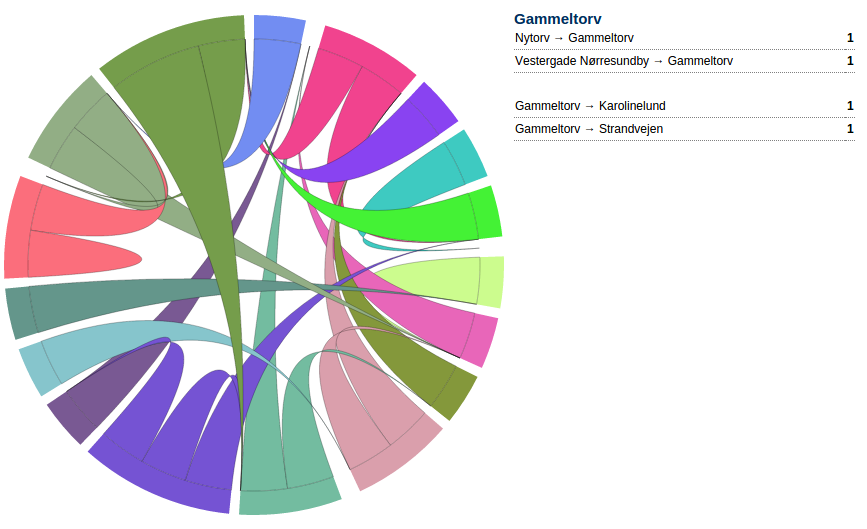
\includegraphics[scale=0.5]{implementation/chorddiagram}
\caption{Chord diagram showing traffic of bicycles.}\label{fig:chorddiagram}
\end{figure}

The timestamp of the event is generated just before query execution, which means that some delay can occur from the actual event firing time to the insertion time, resulting in an imprecise trip duration. 
This is, however, considered a minor deviation in most cases, because the communication delay is short (seconds maybe even less).
In case of a bad connection, the generated timestamp will cause useless data in the light of statistical usage, if time is an important aspect of the analysis.
For showing the traffic between stations the timestamp is used for filtering on a specified time interval and thereby allowing up to an hour of imprecision.
This time interval is an assumed granularity and would have to be specified by the administrator.
The graph showing the amount of bicycles docked at a station shows the timestamp on the x-axis, however, in this case it is considered acceptable with some imprecision since this data will not be used for statistics but for a visual overview.